\section{Annexes}
\subsection{Représentation informatique des objets}
    \begin{center}
    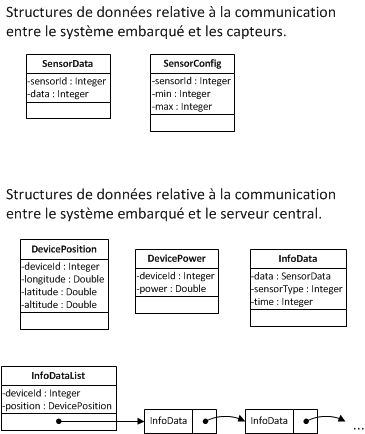
\includegraphics[width=8cm]{\PIXPATH/donnees2}
    \end{center}
	
\subsection{Réflexion sur le réseau}
Nous avons choisi le protocole SSH (Secure Shell) pour les échanges des données entre les systèmes embarqués et le serveur central.  Le protocole de connexion impose un échange de clés de chiffrement en début de connexion. Ce qui assure la sécurité, car il devient impossible d'utiliser un sniffer pour voir les informations échangés. \\

Pour interfacer entre l’utilisateur client et l’application, nous utiliserons un réseau Web, pour cela, le protocole HTTPS (Hypertext Transfer Protocol Secure) assure une communication sûre et chiffrée entre le client et le serveur. \\

    \begin{center}
    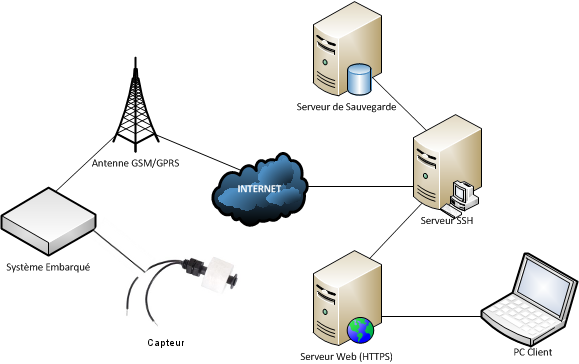
\includegraphics[width=8cm]{\PIXPATH/reseau}
    \end{center}


% Messages...
%\subsection{Réflexion sur le réseau}
% principes qualité, pour la conception du réseau, description du 
% réseau(logiciels, couches, ...)...
%\subsection{Démarrage du système}
% petite réflexion de 1/4 à 1/2 pages max.
